
\input{header}

\hypersetup{
 	pdftitle={01SKEMEU - Příručka ke státnicím},
 	pdfauthor={Martin Kovanda},
 	pdfsubject={Zápisky z přednášek SKE a MEU, FJFI ČVUT},
 	pdfkeywords={Spolehlivost a extrémní události},
 	bookmarksnumbered=true,
 	colorlinks=true,
 	pdfpagemode={UseOutlines}
 }
\makeindex

\title{01SKE + 01MEU}
\date{\today}
\author{01SKE: Bc. Martin Kovanda \& Bc. Jakub Bureš \\ 01MEU: \\  \\
	dle přednášek Ing. Václava Kůse, Ph.D.}

\begin{document}

% ****************************************************************************************************************************
%                             FRONTMATTER
% ****************************************************************************************************************************
\frontmatter
\maketitle

\newpage
\pdfbookmark[0]{Obsah}{obsah}
\tableofcontents

\input{uvod}


% ****************************************************************************************************************************
%                             MAINMATTER
% ****************************************************************************************************************************
\mainmatter
\chapter{[SKE] Spolehlivostní charakteristiky, obecné rodiny hustot, cenzorování, bayesovské odhady v analýze spolehlivosti.}

Budeme pracovat s veličinou  $0\leq T\sim \FT$, která reprezentuje čas do poruchy (\textbf{Failure Time}), třeba do první chyby nebo do uzdravení pacienta. Více se však pracuje s $\RT(t)=1-\FT(t)=\PP(T>t)$ jakožto \textbf{Reliability Function}. Střední doba života (\textbf{Mean Time to Failure}) je vypočtena jako $$\MTTF:=\E T=\int_{0}^{+\infty}\big(1-\FT(t)\big)\d t - \int_{-\infty}^0\FT(t)\d t = \int_{0}^{+\infty}\RT(t)\d t=:\mu.$$

\begin{define}
	\textbf{Mediánový život} $t_\mathrm{med}$ je definován jako $\RT(t_\mathrm{med})=\frac{1}{2}$ a  \textbf{pravý krajní bod} $t_\FF$ jako  $t_\FF=\inf\{ t:\FT(t)\geq1 \}$ ($\RT$ v tomto bodě skočí na nulu a už je dále nula).
\end{define}

\begin{define}
	Intenzitu poruch (FR - \textbf{Failure Rate}) se definuje jako  $\FR(t)=\frac{f_T(t)}{\RT(t)}$.
\end{define}

Význam této veličiny je (úpravou definice) $\FR(t)=\lim\limits_{\Delta t\to 0+}\frac{1}{\Delta t}\PP(t<T\leq t+\Delta t|T>t)$, tedy že výrobek přežil do času $t$ a v následujícím $\Delta t$ čase se pokazí. Tato veličina se definuje, protože je lépe uchopitelná. Může být rostoucí i klesající. Funkce $\RT(t)$ naproti tomu je vždy klesající a pohybuje se v intervalu $[0,1]$.

\begin{theorem}[Vztahy] Platí, že
	$$ \FR(t)=\frac{-\RT(t)}{\RT(t)}=-\frac{\d}{\d t}\big(-\ln \RT(t)\big). $$
	Definujeme \textbf{Cumulative Failure Rate} jako $\Lambda_T(t):= -\ln\RT(t)$. Potom
	$$ \CFR(t) = \int_{0}^{t}\FR(u)\d u. $$
	Dále platí, že 
	$ 1-\FT(t)=\RT(t)=\e{-\CFR(t)} = \e{-\int_{0}^{t}\FR(u)\d u}$. Celkově tedy existuje jednoznačný vztah mezi $\FT$ a $\FR$ za předpokladu spojité distribuční funkce.
\end{theorem}

\begin{figure}[h]
	\centering    
	\begin{tikzpicture}
	\node[inner sep=0pt,anchor=north west] (pic) at (0,0)
	{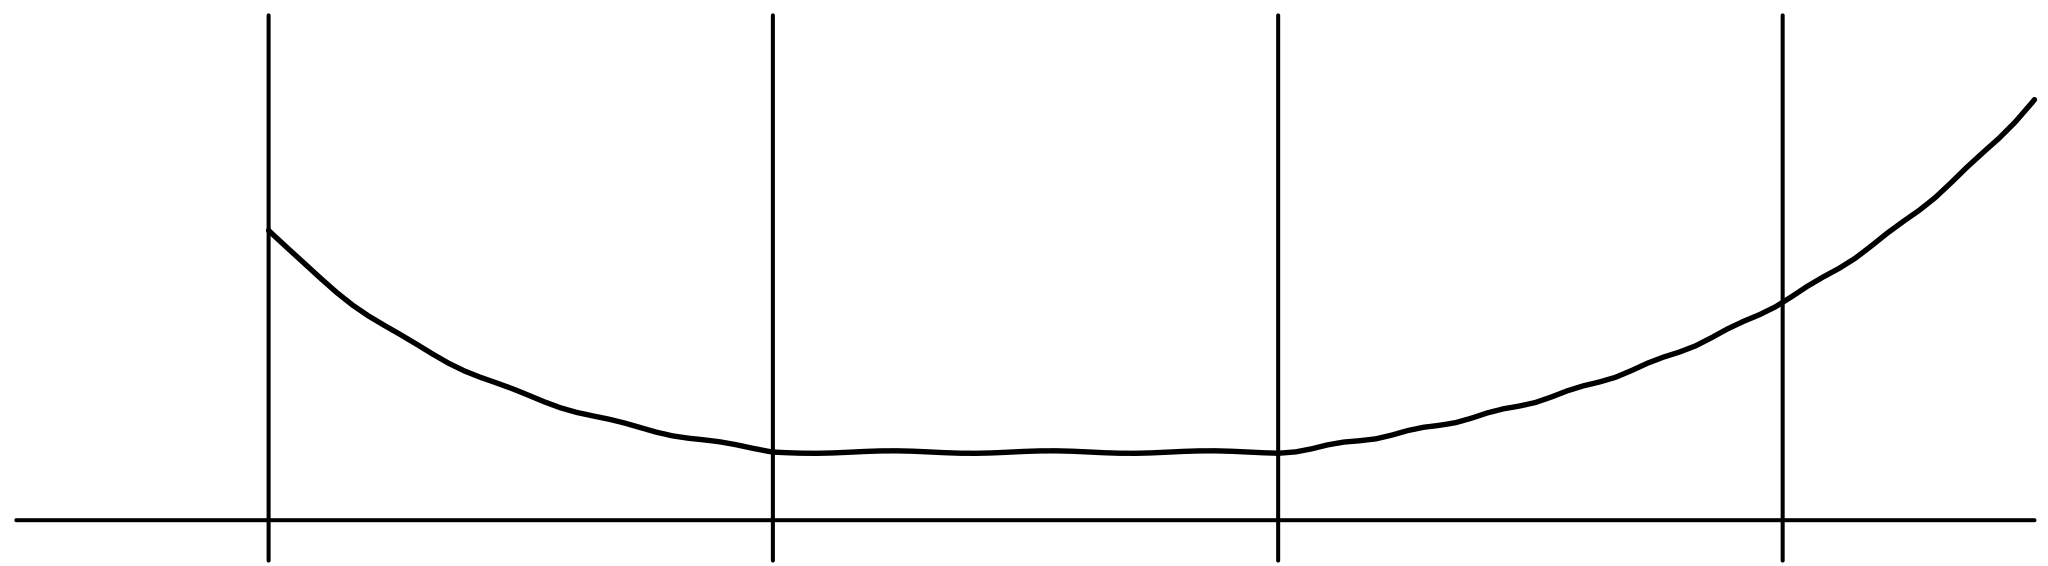
\includegraphics[width=10cm]{pictures/faze.pdf}};
	\draw [color=black](2.36,-0.2) node[anchor=north west] {I};
	\draw [color=black](4.76,-0.2) node[anchor=north west] {II};
	\draw [color=black](7.17,-0.2) node[anchor=north west] {III};
	\draw [color=black](1.3,-1.95) node[anchor=north west] {zajíždění};
	\draw [color=black](3.82,-1) node[anchor=north west] {fáze běžného};
	\draw [color=black](3.82,-1.5) node[anchor=north west] {provozu};
	\draw [color=black](7,-1.95) node[anchor=north west] {stárnutí};
	\draw [color=blue!50!black](0.72,-2.5) node[anchor=north west] {$0$};
	\draw [color=blue!50!black](9.1,-2.5) node[anchor=north west] {$t$};
	\draw [color=blue!50!black](9.2,-1) node[anchor=north west] {$\FR(t)$};
	\end{tikzpicture}
	\caption{Klasický průběh intenzity poruch (technické výrobky apod.).} \label{faze}
\end{figure}

Klasický výrobek se chová podle obr. \ref{faze}. V první fázi se vylaďují výrobní vady, a proto intenzita klesá. Ve druhé fázi je intenzita víceméně konstantní (běžný provoz). V závěrečné fázi materiál stárne a intenzita se zvyšuje.

\begin{define}
Pro $t>0$ definujeme $\RR(x|t):=\PP(T>t+x|T>t)=\frac{\RT(t+x)}{\RT(t)}$ jako \textbf{podmíněná spolehlivost}.	
\end{define}

\begin{define}
Definujeme \textbf{mean residual life} jako $$\MRL(t)=\mu(t)=\int_{0}^{+\infty}\RR(x|t)\d x=\frac{1}{\RT(t)}\int_{t}^{+\infty}\RT(u)\d u.$$
\end{define}

\begin{define}
	Pro $t_2>t_1>0$ definujeme $\RR(t_1,t_2):=\PP(T>t_2|T>t_1)$ jako \textbf{intervalovou spolehlivost}.
\end{define}

\section{Rodiny spolehlivostních modelů}
\begin{define}
	Zavádíme rodinu spolehlivostních modelů \textbf{IFR} (Increasing FR) s rostoucí FR, pokud $\FR(t)$ je rostoucí. Obecněji (pokud by nebyla k dispozici hustota) pak pokud je $\CFR$ konvexní.
	
	Analogicky naopak zavádíme \textbf{DFR} (Decreasing FR).
\end{define}

\begin{define}
	Distribuje $\FF$ je z \textbf{IFRA} rodiny (Increasing RF in Average), pokud $\frac{\CFR(t)}{t}$ je funkce rostoucí na $t>0$.
	
	Analogicky \textbf{DFRA} pro funkci klesající na $t>0$, případně $t\in(0,\t_\FF)$.
\end{define}

\begin{define}
	$\FF$ je z třídy \textbf{NBU} (New Better than Used), pokud $\RR(x|t)\leq\RR(x)=\RR(x|t=0)$, $\forall t>0,\forall x>0$. Analogicky \textbf{NWU} jako New Worse than Used.
\end{define}

\begin{define}
		$\FF$ je z třídy \textbf{NBUE} (New Better than Used in Expectation), pokud $\MRL(t)\leq \MTTF(t)$, $\forall t>0$. Analogicky \textbf{NWUE}.
\end{define}

\begin{theorem}
	$\IFR\Rightarrow\IFRA\Rightarrow\NBU\Rightarrow\NBUE$.
\end{theorem}

\section{Cenzorovaná data}
Doteď se pracovalo s úplným výběrem. Měli jsme tedy $n$ $iid$ objektů a pozorovaly se všechny časy do poruchy. Nyní se však pracuje s živými objekty (lidmi, zvířaty apod.), které se mohou rozhodnout pozorování opustit. Může se například cenzorovat časem, tj. experiment se ukončí po nějakém čase. Může se cenzorovat i počtem poruch, tj. experiment je ukončen po $r$-té poruše. Třetí možností je cenzorovat náhodně. Každý pocient je tedy cenzorován jeho vlastním cenzorovaným časem, což je náhodná veličina s $\FF_C$.

\begin{example}
	Exponenciální rozdělení $T\sim\Exp(\lambda)$ má následující vlastnosti:\begin{enumerate}
		\item $f_T(t)=\lambda\e{-\lambda t}$, $\RT(t)=\e{-\lambda t}$, $\CFR=\lambda t$, $\RR(x|t)=\e{-\lambda t}$, $\FR(t)=\lambda$
		\item $\MTTF=\frac{1}{\lambda}$, $\MRL(t)=\MTTF$
		\item celkově tedy IFR=DFR, IFRA=DFRA, NBU=NWU
	\end{enumerate}
\end{example}
\begin{theorem}[Smirnoffova transformace]
	Mějme čas do poruchy $T\sim\RT$, $\widetilde{T}:=\CFR(T)=-\ln\RT(T)$. Pak $\widetilde{T}\sim\Exp(1)$ s $\lambda_{\widetilde{T}}=1$ konstantní (tedy nestárne, ani nemládne, což vyplývá z vlastností exponenciálního času do poruchy). Navíc platí, že $T=t\Leftrightarrow \widetilde{T}=\CFR(t),~\forall t>0$ (pro spojité modely).
\end{theorem}

\section{Bayesovské odhady v analýze spolehlivosti}

\begin{define}[Gamma rozdělení]
	Mějme $T|\lambda\sim \Exp(\lambda)$ u nestabilní výroby ($\lambda=\lambda(t)$). Zde se vyplatí použít nějaké apriorní informace o $\lambda$, tedy $\lambda\sim\pi(\lambda)=\mathrm{Gamma}(k,\beta)$. Potom
	$$ \RT(t)=\int_{t}^{+\infty}f_T(u)\d u=\int_{t}^{+\infty}\int_{0}^{+\infty}\Exp(\lambda)\mathrm{Gamma}(k,\beta)\d\lambda\d u =\int_{0}^{+\infty}\mathrm{Gamma}(k,\beta)\RR_{T|\lambda}(t)\d\lambda=\frac{\beta^k}{(\beta+t)^k}, $$
	což je Paretovo rozdělení (s těžkým chvostem). Dále platí, že $\FR(t)=\frac{k}{\beta+t}$, což je klesající funkce, takže se toto rozdělení hodí např. pro modelování první fáze výrobku.
\end{define}

\begin{example}
	Jiná možnost by byla pro $(T_1...T_n)~iid~T|\lambda\sim\Exp(\lambda)$, $\lambda\sim\mathrm{Gamma}(k,\beta)$ odhadnout parametr $\lambda$ bayesovsky a dosadit ji do $\E T|\lambda$. Parametry $(k, \beta)$ lze nalézt např. pomocí empirického Bayese.
\end{example}



\chapter{[SKE] Parametrické modely s (ne)monotónní intenzitou poruch, únavové cyklické zkoušky, příklady použití.}

\begin{define}[Normální rozdělení]
	Mějme $T\sim \NN(\mu, \sigma^2)$ (kde zanedbáme zápornou část, tedy chceme $\mu$ dostatečně daleko od nuly). Platí, že 
	$$ \FR(t)=\frac{\frac{1}{\sigma}\phi\big(\frac{t-\mu}{\sigma}\big)}{1-\Phi\big(\frac{t-\mu}{\sigma}\big)}.$$
		Dále se může použít useknuté normální rozdělené v $t=0$ zleva $\mathcal{TN}(\mu,\sigma^2)$, tedy $$\RT(t)=\frac{\PP(T>t)}{\PP(T>0)}=\frac{1-\Phi\big(\frac{t-\mu}{\sigma}\big)}{1-\Phi\big(\frac{\mu}{\sigma}\big)}.$$ Pro $t>0$ je $\FR(t)$ shodná s předešlým případem.
\end{define}

Normální rozdělení se tedy dá použít na modelování třetí fáze opotřebování výrobku.

\begin{define}[Gamma rozdělení]
Mějme $T_i\sim \Exp(\lambda)$. Pak $T:=\sum_{1}^{k}T_j$ je čekací doba na výskyt $k$-té poruchy (třeba pokud máme $k$ náhradních dílů). Tím dostáváme $T\sim\mathrm{Gamma}(k,\lambda)$. $\lambda>0$ nazýváme \textbf{intenzita šoků} a $k>0$ míru rezistence. Víme dále, že $\MTTF=\E T=\frac{k}{\lambda}$. 
\end{define}

\begin{define}[Weibulovo rozdělení]
	Definujeme \textbf{Weibulovo} rozdělení definováno vztahem $\RT(t)=\e{-(\lambda t)^\alpha}$, tedy $f_T(t)=\alpha \lambda^\alpha t^{\alpha-1}\e{-(\lambda t)^\alpha}$. Platí, že
	$$ \FR(t)=\alpha\lambda^\alpha t^{\alpha-1},~\MTTF=\frac{1}{\lambda}\Gamma\big(1+\frac{1}{\lambda}\big),~t_\mathrm{med}=\frac{1}{\lambda}(\ln2)^{1/\alpha}.$$
\end{define}




\chapter{[SKE] Spolehlivost komponentních systémů, redundantní struktury, důležitost komponent.}

% lecture 7
    \begin{define}
        Předpokládejme, že máme systém o $n$ komponentách. Budeme charakterizovat stav $i$-té komponenty $x_i$ binárně jako funguje/nefunguje, tedy $x_i\in\{0,1\}$. Označme $\textbf{x}=(x_1,...,x_n)$ jako \textbf{stavový vektor}. 
        
        Předpokládejme, že známe-li $\textbf{x}$, pak známe stav celého systému $S$, tzn. jsme schopni definovat \textbf{strukturní funkci} $\crossedphi(\textbf{x})=\begin{cases}
        1,&\text{systém funguje,}\\0,&\text{systém nefunguje.}
        \end{cases}$
    \end{define}

    Tímto způsobem můžeme zkoumat různě zapojené součásti, třeba sériově, 
    paralelně (jsou tedy v redundanci) apod. U sériového zapojení stačí 
    jedna vadná součástka, aby systém přestal fungovat a u paralelního 
    systému stačí, když alespoň jedna součástka funguje, aby systém 
    fungoval. Pozor ale, že záleží na reprezentaci, někdy se např. sériově 
    zapojené součástky chovají, jako by byly paralelní (např. ventily na 
    potrubí, aby voda netekla, alespoň jeden ventil musí fungovat).

    \begin{corollary}
        Logické zapojení komponent se může zakreslit pomocí blokových diagramů (RBD - Reliability Block Diagram) (podobné elektrickému zapojení). Pro sériově zapojené součásti máme 
        $$ \crossedphi(\textbf{x})=\prod_{i=1}^{n}x_i=\min(x_i)_1^n.$$
        Paralelně zapojené součástky pak
        $$ \crossedphi(\textbf{x})=1-\prod_{i=1}^{n}(1-x_i)\equal{ozn}\bigsqcup_{i=1}^n x_i=\max(x_i)_1^n, $$ kde $\bigsqcup$ označuje inverzní produkt.
    \end{corollary}

    \begin{define}[k-o-o-n struktura]
        k-o-o-n struktura (k-out-of-n) je taková, že systém funguje, pokud je alespoň $k$ z komponent je funkční. Potom
        $$ \crossedphi(\textbf{x})=\begin{cases}
        1,&\text{pokud }\sumin x_i\geq k,\\0,& \text{jinak.}
        \end{cases}$$
        Tento systém se může použít třeba pro přivolávání hasičů, pokud 2oon zaznamenají kouř. Tímto se eliminují false positive chyby ve stylu zapálená cigareta apod. Například systém 2oo3 se dá zapsat jako paralelní vlákna $\{(1,2), (2,3),(1,3)\}$. Není to však jediná možnost, viz obrázek \ref{fig:2oo3}.
        
        \begin{figure}[h]
            \centering
            \includegraphics[width=0.7\linewidth]{pictures/2oo3}
            \caption{Dvě možnosti zapojení systému 2oo3, paralelní systém minimálnních cest (vlevo) a série minimálních řezů (vpravo).}
            \label{fig:2oo3}
        \end{figure}
        
        Máme tedy $\crossedphi(\textbf{x})=x_1x_2\bigsqcup x_1x_3\bigsqcup x_2x_3$
    \end{define}

    \begin{theorem}
        Mějme systém S o $n$ komponentech. Mějme dále minimální cesty $P_1,...,P_k$ (funkční cesty ze kterých nelze nic odstranit). Pak $$ \crossedphi(\textbf{x})=\bigsqcup_{j=1}^k \prod_{i\in P_j} x_i.$$
        Naopak z minimálních řezů $K_1,...,K_l$ můžeme dostat
        $$ \crossedphi(\textbf{x})= \prod_{j=1}^k \bigsqcup_{i\in K_k} x_i.$$
        V praxi pak používáme ten vzorec, který nejvíce zjednodušuje výpočet.
    \end{theorem}

    \begin{corollary}
        Definujeme strukturu BRIDGE (viz obr. \ref{fig:bridge}). Tady máme 4 cesty, kudy projít, tedy $\{(1,2),(4,5),(1,3,5),(4,3,2)\}$. Z toho můžeme udělat $\crossedphi(\textbf{x})$. Poměrně jednoduše se dá udělat i diagram řezů.
        
        \begin{figure}[h]
            \centering
            \includegraphics[width=0.3\linewidth]{pictures/bridge}
            \caption{Strukture BRIDGE.}
            \label{fig:bridge}
        \end{figure}
        
    \end{corollary}

    \begin{theorem}[Pivotální rozklad]
        Mějme systém $S$ o $n$ komponentách. Pak můžeme $\crossedphi(\textbf{x})$ rozepsat jako 
        $$\crossedphi(\textbf{x})=x_i\crossedphi(1_i,\textbf{x}_{-i})+(1-x_i)\crossedphi(0_i,\textbf{x}_{-i}),$$
        kde fixujeme, že $i$-tý prvek funguje/nefunguje. Tento rozklad se může použít rekurentně až do 
        $$\crossedphi(\textbf{x})=\sum_{\textbf{y}}\prod_{j=1}^n x_j^{y_j}(1-x_j)^{1-y_j}\crossedphi(\textbf{y}),$$ kde $\textbf{y}$ jsou $n$-rozměrné binární vektory, kterých je $2^n$.
    \end{theorem}

    Toto se hodí např. pro BRIDGE, kde je ideální udělat rozklad podle prvku 3. Potom dostaneme 
    $$ \crossedphi(\textbf{x})=x_3\crossedphi(1_3,\textbf{x}_{-3})+(1-x_3)\crossedphi(0_3,\textbf{x}_{-3}). $$ 
    Tím se výrazně zjednoduší struktura systému.

    \begin{define}[Strukturní důležitost komponent]
        Stavový vektor $(1_i,\textbf{x})$ se nazývá \textbf{kritická cesta/vektor pro $i$-tou komponentu}, pokud $\crossedphi(1_i,\textbf{x})=1\wedge \crossedphi(0_i,\textbf{x})=0 $, tzn. $\crossedphi(1_i,\textbf{x})-\crossedphi(0_i,\textbf{x})=1$.
        
        Označme $\eta_\crossedphi(i)=\sum_{(\cdot_i,\textbf{x}_{-i})} \big[\crossedphi(1_i,\textbf{x})-\crossedphi(0_i,\textbf{x})\big]$ počet kritických vektorů pro $i$-tou komponentu.
        
        Číslo $B_\crossedphi(i)=\frac{\eta_\crossedphi(i)}{2^{n-1}}$ nazveme \textbf{Birmbaumova míra (strukturní) důležitosti} $i$-té komponenty v $S$.
    \end{define}

    \begin{example}
        Komponenta 1 je v sérii s paralelní 2 a 3. Pak pro $i=1$ dostaneme
        $$\begin{array}{c|c}
            (\cdot,x_2,x_3) & \crossedphi(1_i,\textbf{x})-\crossedphi(0_i,\textbf{x})=1 \\\hline
            \cdot\,00 & 0 \\
            \cdot\,01 & 1 \\
            \cdot\,10 & 1 \\
            \cdot\,11 & 1 
        \end{array}.$$
        Jelikož $2^{n-1}=4$, pak $\eta_\crossedphi(1)=3$, takže $B_\crossedphi(1)=\frac{3}{4}$ apod.
        
    \end{example}


    \begin{define}
        $i$-tá komponenta se nazývá \textbf{irelevantní}, pokud $\crossedphi(1_i,\textbf{x})=\crossedphi(0_i,\textbf{x})$, $\forall\textbf{x}_{-i}$. Tedy že na jejím vypnutí/zapnutí nezáleží. Příkladem je záznamové zařízení při požárním poplachu, které je sice důležité, ale na samotný poplach nemá vliv.
    \end{define}

    \begin{define}
        Systém komponent se nazývá \textbf{koherentní}, pokud neobsahuje irelevantní komponenty a strukturní funkce je neklesající v každé své proměnné.
    \end{define}

    \begin{theorem}
        Pro $S$ koherentní platí, že $\crossedphi(\textbf{0})=0$, $\crossedphi(\textbf{1})=1$ a $$ \prod_{i=1}^n x_i\leq \crossedphi(\textbf{x})\leq \bigsqcup_{i=1}^n x_i. $$
    \end{theorem}

    \begin{define}[Spolehlivostní funkce]
        Pro výpočet $R_S(t)$ využijeme čas $t$ a ztotožníme poruchovostní komponenty 
        $$X_i(t)=\begin{cases}1,&\text{s pravděpodobností }p_i=\PP(T_i>t),\\0,&\text{jinak.}\end{cases}$$
        Dosazením do strukturní funkce potom vyrobíme $\crossedphi\big(\textbf{X}(t)\big)$, kde $\textbf{X}(t)$ je vektor veličin $X_i(t)$, které charakterizují funkčnost/nefunkčnost komponenty v čase $t$. Potom
        $$ R_S(t)=\PP(T_S>t)=\PP\big(\crossedphi\big(\textbf{X}(t)\big)=1\big)=1\cdot\PP\big(\crossedphi\big(\textbf{X}(t)\big)=1\big)+0\cdot\PP\big(\crossedphi\big(\textbf{X}(t)\big)=0\big)=\EE{\crossedphi\big(\textbf{X}(t)\big)}. $$
    \end{define}

    \begin{example}
        Pro sériově zapojený $S$ dostaneme
        $$ R_S(t)=\E \crossedphi\big(\textbf{X}(t)\big)\equal{id}\prod_{i=1}^n \E X_i(t)=\prod_{i=1}^n R_i(t)=\prod_{i=1}^n \e{-\int_{0}^{t}\lambda_i(\tilde{t})\d\tilde{t}}=\e{-\int\limits_{0}^t\sumin \lambda_i(\tilde{t})\d\tilde{t}}, $$
        kde $\sumin \lambda_i(\tilde{t})\d\tilde{t}=\lambda_S(\tilde{t})$. Z toho vyplývá, že např. pro 100 komponent o $R_i(t)=0.995$ dostaneme systém o spolehlivosti $R_s(t)=0.606$. Sériové systémy jsou tedy nejhorší možné, co se týče spolehlivosti. 
    \end{example}

    \begin{example}
        Pomocí tří imaginárních komponent (DFR,CFR,IFR) jde modelovat fyzická (reálná) komponenta s vanovitým průběhem FR. U paralelních součástí máme naopak 
        $$ R_S(t)=\E\crossedphi\big(\textbf{X}(t)\big)=\E\Big[\bigsqcup_{i=1}^n X_i(t)\Big]=\E\Big[1-\prod_{i=1}^n(1-X_i(t))\Big]\equal{id}1-\prod_{i=1}\big(1-R_i(t)\big)=\bigsqcup_{i=1}^n R_i(t). $$
    \end{example}

    \begin{example}
    S je k-o-o-n: 
    $$ R_S(t)=\E\crossedphi\big(\textbf{X}(t)\big)= \PP\big(\sum_{i=1}^n X_i(t)\geq k\big)\equal{iid}\sum_{x=k}^n {n\choose x} R(t)^{x} (1-R(t))^{n-x} = \sum_{x=k}^n {n\choose x} \e{-\lambda tx} \big(1-\e{-\lambda t}\big)^{n-x}   $$
    Z čehož můžeme potom získat střední dobu do poruchy
    $$\MTTF_S = \sum_{x=k}^n {n\choose x} \int_0^\infty \e{-\lambda tx} \big(1-\e{-\lambda t}\big)^{n-x} \d t = \Bigg| \e{-\lambda t} = y \Bigg| = \dots =  \frac{1}{\lambda} \sum_{x=k}^n \frac{1}{x},$$
    kde jsme využili substice, která integrál převede na beta funkci a dále se dá zjednodušit do výše uvedeného tvaru. V tabulce jsou uvedeny konkrétní případy $\MTTF$ pro různá $k$ či $n$.

    \begin{table}[h]
        \centering
        \begin{tabular}{|l|l|l|l|l|}
            \hline
            $k$\textbackslash $n$& 1 & 2 &3  & 4 \\ \hline\hline
            1&$\frac{1}{\lambda}$  &  $\frac{3}{2}$$\frac{1}{\lambda}$& $\frac{11}{6}$$\frac{1}{\lambda}$ & $\frac{25}{12}$$\frac{1}{\lambda}$ \\ \hline
            2& $\times$ & $\frac{1}{2}$$\frac{1}{\lambda}$ & $\frac{5}{6}$$\frac{1}{\lambda}$ &  \\ \hline
            3&  &  & $\frac{1}{3}$$\frac{1}{\lambda}$ &  \\ \hline
            4&  &  &  & $\frac{1}{4}$$\frac{1}{\lambda}$ \\ \hline
        \end{tabular}
    \end{table}
    \end{example}

\section{Redundance}

    \begin{theorem}
        Mějme $n$-komponentní systém $S$ a stavové vektory $\textbf{x}$, $\textbf{y}$. Potom pro koherentní strukturu S platí $\crossedphi(\textbf{x} \bigsqcup \textbf{y}) \geq  \crossedphi(\textbf{x}) \bigsqcup \crossedphi(\textbf{y})$.
    \end{theorem}

%lecture 9

    V této úloze řešíme, jakým způsobem lze uchopit zálohu nějaké části systému.

    \subsection*{Aktvní záloha}
    
    Aktivní záloha je pararelní záloha části systému a je v plném provozu a může se tedy porouchat. Tyto systémy json obyčejné paralelní systémy, které jsme doposud dělali. Můžeme tedy spočítat $R_S$, $\lambda_S$, $\MTTF_S$, apod.
    
    \subsection*{Pasivní záloha + perfect switch}
    
    Rezervní komponenta čeká ve stand-by režimu a její rozbití v tomto čase zanedbáme. V této úloze máme switch, který musí být schopný zařadit do systému rezervní komponentu.
    Pokud počítáme s perfektně fungujícím switchem, potom se dá vypočítat $T_S = \sum_{i=1}^n T_i$, $\MTTF = \sum_{i=1}^n \MTTF_i$, $R_S(t) = \PP\Big(\sum_{i=1}^n T_i\Big) = \otimes_{i=1}^n R_i(t)$ a pro dostatečně velké $n$ je $\sum_{i=1}^n T_i $ asymptoticky normální nebo $AG_{\alpha}$.
    
    \subsection*{Pasivní záloha + imperfect switch}
        Zde charakterizujeme switch pomocí pravděpodobnosti, tedy pravděpodobnost, že switch skutečně přepne na záložní komponentu, je 1-$p$. 
        Předpokládáme navíc, že komponenty včetně switche jsou nezávisle fungující. Mohou nastat 2 případy.
            \begin{enumerate}
                \item Komponenta 1 drží až do času t, to nastane s pravděpodobností $R_1(t)$.
                \item Komponenta 1 se porouchala v určitém čase v $(0,t)$, když označíme $\tau < t$ jako čas poruchy,tak se komponenta 1 porouchala v $(\tau,\tau + \d\tau)$. Pravděpodobnost, že nastane tato situace se dá jednoduše zapsat jako hustota $f_{T_1}(\tau)\d\tau$ $\longrightarrow$ Switch přepne s pravděpodobností 1-$p$ v čase $\tau$ $\longrightarrow$ Komponenta 2 je nyní aktivní v čase $\tau$ a funguje až do $t$. Toto nastane s pravděpodobností $R_2(t-\tau)$.
            \end{enumerate}
    Podívejme se nyní na pravděpodobnost, že je celý tento systém $S$ funkční. Platí, že
    \begin{align*}
        \PP\big(\text{ je OK v čase }t \big) =  & \PP(T_S > t ) = R_S(t) = \PP(\mathrm{i.}) + \PP(\mathrm{ii.}) = \\ &
        R_1(t) + \int_0^t (1-p)R_2(t-\tau) f_{T_1}(\tau)\d\tau = \\ &
        \e{-\lambda_1 t} + \int_0^t (1-p)\e{-\lambda_2 (t-\tau)} \lambda_1\e{-\lambda_1 \tau}  \d\tau = \\ &
        \e{-\lambda_1 t} + \frac{(1-p)\lambda_1}{\lambda_1-\lambda2}\e{-\lambda_2 t} - \frac{(1-p)\lambda_1}{\lambda_1-\lambda2}\e{-\lambda_1 t}.
    \end{align*}
    Navíc můžeme také určit 
    \begin{align*}
        \MTTF_S = \int_0^{\infty} R_S(t) \d t = \frac{1}{\lambda_1} + \frac{1-p}{\lambda_2}.
    \end{align*}

    \subsection*{Částečná záloha + imperfect switch}
    
    Rezervní komponenta je pod minimálním zatížením a může se tedy porouchat.  Máme $T_1$ se spolehlivostí $R_1$, $T_2$ se spolehlivostí $R_2$ a switch, který přepíná s pravděpodobností $(1-p)$. Navíc máme $T_0 \sim R_0$, což je doba do poruchy komponenty 2 v době minimálního zatížení. Obdobně lze rozdělit na dva případy.
    \begin{enumerate}
        \item Komponenta 1 drží až do času t, to nastane s pravděpodobností $R_1(t)$.
        \item Komponenta 1 se porouchala v určitém čase v $(0,t)$, když označíme $\tau < t$ jako čas poruchy,tak se komponenta 1 porouchala v $(\tau,\tau + \d\tau)$. Pravděpodobnost, že nastane tato situace se dá jednoduše zapsat jako hustota $f_{T_1}(\tau)\d\tau$ $\longrightarrow$ Switch přepne s pravděpodobností 1-$p$ v čase $\tau$ $\longrightarrow$ Komponenta 2 není porouchána v čase $\tau$, nastává s pravděpodobností $R_0(\tau)$ $\longrightarrow$ Komponenta 2 je funkční v čase $t$, tzn. $R_2(t-\tau)$.
    \end{enumerate}
    
    Máme tudíž o jednu variantu navíc, než v předchozím případě. Opět lze určit 
    \begin{align*}
        R_S(t) = &	R_1(t) + \int_0^t (1-p)R_0(\tau)R_2(t-\tau) f_{T_1}(\tau)\d\tau = \\ &
        \e{-\lambda_1 t} + \frac{(1-p)\lambda_1}{\lambda_0+\lambda_1-\lambda_2}\big(\e{-\lambda_2 t} - \e{-(\lambda_0 + \lambda_1) t} \big)
    \end{align*}
    a
    \begin{align*}
        \MTTF_S = \int_0^{\infty} R_S(t) \d t = \frac{1}{\lambda_1} + \frac{1-p}{\lambda_2} - (1-p)\frac{\lambda_0}{\lambda_2(\lambda_1 + \lambda_0)}.
    \end{align*}
    
\section{Extreme Value Distribution (EVD)}

    V této části budeme počítat spolehlivost pro extrémní události. Budeme tedy zkoumat, jak jsou rozloženy minima a maxima nějaké iid posloupnosti pozorování. To ale přesně odpovídá tomu, co se probíralo v minulých sekcích pro sériové a paralelní systémy.

    \begin{define}[Gumbelovo rozdělení (sériový systém)]
        Nechť $T_j \sim f_T(t) = o\big(\e{-\beta\abs{t}} \big)$ (exponenciální chvosty) při $t \rightarrow \infty$, ale není useknuté zleva (např. Gauss, ale ne Pareto). Pak 
        $$ U_n:=\min(T_j)_1^n  \Dto Y  ,$$ kde
        pro distribuční funkci náhodné veličiny $Y$ platí, že	
        $$ \FF_Y(t)  = 1 - \e{-\exp(\frac{t-\vartheta}{\alpha} )},~~t \in \R, \vartheta \in \R, \alpha \in\R^+,  $$
        což se nazývá \textbf{Gumbelovo rozdělení} (extreme value distribution type 1).
    \end{define}
    
    Toto rozdělení se hodí pro modelování III části pro výrobky, kde je možné předpokládat dokonce exponenciální nárůst intenzity poruch. Takovéto výrobky spadají také do tzv. Gompertz-Makehamova zákona. Ten říká, že pravděpodobnost smrti roste exponenciálně s věkem.

    \begin{define}[Gumbelovo rozdělení (paralelní systém)]
        Nechť $T_j \sim f_T(t) = o\big(\e{-\beta\abs{t}} \big)$ (exponenciální chvosty) při $t \rightarrow \infty$, ale není useknuté zprava (prakticky vždy vyhovuje). Pak 
        $$ M_n:=\max(T_j)_1^n  \Dto Y  ,$$ kde
        pro distribuční funkci náhodné veličiny $Y$ platí, že	
        $$ \FF_Y(t)  = \e{-\exp(-\frac{t-\vartheta}{\alpha} )},~~t \in \R, \vartheta \in \R, \alpha \in\R^+,  $$
        což se nazývá \textbf{Gumbelovo rozdělení} pro maximum.
    \end{define}
    

\chapter{[SKE] Odhady spolehlivosti a kumulativní intenzity poruch, typy cenzorování, testy.}


\subsubsection{Pararelní systém n-komponentní}
$$T_S = \max{\big(T_j\big)_{i=1}^n} =  M_n$$\\
$$R_S(t)\equal{id} 1 -  \prod_{j=1}^n R_j(t) \equal{iid}  1 - \big(1 -R_T(t) \big)^n$$ \\
$$\FF_S(t) \equal{iid} \big(\FF_T(t)\big)^n$$

Můžeme formulovat obdobnou větu jako pro sériový systém.

\begin{theorem}
	Nechť $T \sim f_T(t) = o\Big(\e{-\beta\abs{t}} \Big)$ při $t \rightarrow \infty$, ale není useknuté zprava. Pak 
	$$M_n  \Dto Y  ,$$ kde
	pro distribuční funkci náhodné veličiny $Y$ platí
	
	$$ \FF_Y(t)  = 1 - \e{-\exp(\frac{t-\vartheta}{\alpha} )},~~t \in \R, \vartheta \in \R, \alpha \in\R^+.  $$
\end{theorem}

\subsection{Model konkurenčních rizik, Competing risks}
Nechť je $T$ doba do poruchy. Ta může nastat z různých příčin, označme je jako $\delta \in \lbrace1,2,\dots k \rbrace$. Máme tedy $k$ módů rizika/poruchy, které soutěží o vyřazení komponenty - proto Competing risks. Široká škála využití v praxi, například demografie, či sociologie. 
\begin{example}
	Pro představu uveďme několik příkladů. $T$ může být například doba trvání manželství, nezaměstnanosti nebo nemoci. V ekonomii se může jednat o dobu do krachu firmy. Ve stavitelství se můžeme bavit o době do pádu určitého mostu, atd.	
\end{example}
Reprezentujme to pomocí dvojce $(T, \delta)$, kde jsou oba prvky náhodnými veličinami, navíc $T \geq 0$ a $\delta\in\hat{k}$. Tato dvojce má sdruženou distribuční funkci $(T, \delta) \sim \FF_{T,\delta}(t,d)$, kde $t\in\R, d\in \R$. Tato distribuční funkce je ovšem v $d$ diskrétní, čili v proměnné $d$ se nachází skoky. Nyní $\FF_{T,\delta}(t,d)$ charakterizujme pomocí subdistribucí.
$$R(t,j) = \PP(T > t, j)~~t \in \R, ~~j \in \hat{k}$$ 
$$p_j = \PP(\delta = j) = R(0,j), ~~\sum_{k=1}^n p_k = 1$$ 
Budeme potřebovat také subhustoty, které definujeme předpisem $f(t,j)=R'(t,j)$. Pomocí tohoto objektu lze určit hustota marginální hustota pro $T$, či disitribuční a spolehlivostní funkce.
$$f_T(t) = \sum_{i = 1}^{n}f(t,j)$$
$$\FF_T(t) = \int_{-\infty}^{t} \sum_{j=1}^n f(y,j)\d y = \sum_{j=1}^n \FF(t,j)  $$
$$R_T(t) = \int_{t}^{\infty} \FF(y,j) \d y = \sum_{j=1}^n R(t,j) $$
$$r_T(t) = \frac{f_T}{R_T} = \sum_{j=1}^n\frac{f(t,j)}{R_T} = \sum_{j=1}^n r_T(t,j) $$
Můžeme definovat také relativní intenzitu poruch $j$-tého módu rizika $\frac{r_T(t,j)}{r_T(t)}$.
Pokračujme definováním dalších veličin.
$$ R_T(t|j) = \PP(T > t|\delta =j) = \frac{\PP(T > t, \delta =j)}{\PP(\delta =j)} = \frac{R(t,j)}{p_j} $$
$$R_T(t) = \sum_{j=1}R(t,j) = \sum_{j=1}p_j R_T(t|j)$$
V poslední rovnosti jsme získáli $R_T(t)$ jako konvexní směs podmíněných distribucí. Povšivněme si však, že jsme nikde nepředpokládali vzájemnou nezávislost konkurenčních rizik. Tyto vztahy platí i v přípádě, že jednotlivé módy rizika jsou na sobě závíslé.
\subsection{LIFE-TIME aplikace}
Budeme využívat tzv. \emph{Censoring} dat. Censorovat data můžeme několika způsoby.

\paragraph{Censorování typu I.} Experiment ukončíme v čace $t_c$. Data jsou tvaru $T_{(1)},T_{(2)},\dots, T_{(r)} \leq t_c$, přičemž máme informaci, že $T_{(r+1)},T_{(r+2)},\dots, T_{(n)} \geq t_c$. Lze zapsat také následovně 

$$W_j = \min(T_j,t_c) = \begin{cases}
	T_j,& T_j\leq t_c,\\ t_c,& otherwise
\end{cases}, ~~\delta_j = I\lbrace T_j \leq t_c \rbrace = \begin{cases}
	1\\ 
	0
\end{cases}$$. \\
V následující větě se podíváme jak se dá sestrojit vztah pro hustotu pravděpodobnosti prvních $r$ uspořádaných statistik, včetně $r$, které je náhodné.
\begin{theorem}
	Nechť $T_1, T_2, \dots, T_n$ jsou i.i.d. s příslušnou distribuční funkcí $\FF$ či hustotou $f$. Označme $T_{(1)} < T_{(2)} < \cdots <T_{(r)}$, kde $r\in\hat{n}$. Pak $$f(t_1, t_2, \dots, t_n| r) = \frac{n!}{(n-r)!}\Big(\prod_{j=1}^r f(t_{(j)})\Big)R(t_c)^{n-r}, ~~ \forall t_{(1)} < t_{(2)} < \cdots <t_{(r)} \leq t_c $$ 
	a navíc
	$$f(t_1, t_2, \dots, t_n r) = \frac{r!}{\FF^r(t_c)}\prod_{j=1}^r f(t_{(j)}) = r! \prod_{j=1}^r  \frac{f(t_{(j)})}{\FF(t_{c})}, ~~ t_{(j)} \leq t_c$$ 
\end{theorem}

\paragraph{Censorování typu II.}
Také se jinak nazývá censorování poruchou. V tomto typu censoringu volíme $r$ pevně a čas experimentu (zde označme $t_{\mathrm{exp}} = t_{(r)}$) je náhodná veličina. Data pak vypadají takto: 
$$W_j = \min(T_j, t_{(r)})_{j=1}^n = \begin{cases}
	T_j,& T_j\leq t_{(r)},\\ t_{(r)},& otherwise
\end{cases},~~\delta_j = I\lbrace T_j \leq t_{(r)} \rbrace = \begin{cases}
	1\\ 
	0
\end{cases}
$$
I zde můžeme formulovat podobnou větu, jako v případě Censoringu typu I.
\begin{theorem}
	Nechť $T_1, T_2, \dots, T_n$ jsou i.i.d. s příslušnou distribuční funkcí $\FF$ či hustotou $f$. Označme $T_{(1)} < T_{(2)} < \cdots <T_{(r)}$, kde $r\in\hat{n}$. 
	Pak $$f(t_1, t_2, \dots, t_n| r) = \frac{n!}{(n-r)!}\Big(\prod_{j=1}^r f(t_{(j)})\Big)R(t_{(r)})^{n-r}, ~~ \forall t_{(1)} < t_{(2)} < \cdots <t_{(r)} \leq t_c $$ 
	
\end{theorem}
\paragraph{Censorování typu III.}
Kombinace přechozích dvou censorování, tedy nastavíme pevně čas experimentu $t_c$ a také nastavíme pevně $r$.
%lecture 10
\paragraph{Random censoring, RC.}
Máme opět čas do poruchy $T$, navíc máme ovšem další náhodnou veličinu $C$, kterou nazveme časový cenzor. Oěb tyto veličiny jsou výájemně nezávislé. Distribuční funkce těchto náhodných veličin jsou pro jasnost $\FF_T$ a $\FF_C$. Časový cenzor realizuje censorování každé jednotlivé časové hodnoty. Data v tomto případě zapisujeme ve tvaru

$$W = \min(T,C), ~~\delta_j = I\lbrace T \leq C \rbrace = \begin{cases}
	1& T\leq C,\\0& T > C 
\end{cases}
$$
Čímž dostáváme opět spojitě diskrétní rozdělení pro dvojici
$(W,\delta)$ v modelu konkurenčních rizik. Tím máme hotový setup modelu. Podívejme se jak vypadá střední hodnota
$$q = \EE{\delta} =  \EE{I\lbrace T \leq C \rbrace} = \int_{\lbrace T \leq C \rbrace}1\d\PP = \PP(T\leq C)\equal{id} = \iint_{t\leq c}\d\FF_T\d\FF_C = \iint_{t\leq c}f_Tf_C  \d t \d c$$
Víme-li, že máme k dispozici $n$ pozorování, potom číslo $n\cdot q$ značí střední počet poruch v $n$-tici opakování. \\
Zaznamenáváme $T_j, C_j$, což vede na data ve tvaru $(W_j,\delta_j)_{j=1}^n$. Dále označme $D$ množinu indexů, kdy opravdu došlo k poruše, čili $$D = \lbrace j\in \hat{n}: \delta_j =1 \rbrace .$$ Často nazývána také jako množina defektů. Mohutnost množiny $\abs{D} = \# D = \delta = \sum_{j=1}^n\delta_j$, tedy počet poruch v $n$-tici. Tímto censoringu se budeme zejména zabývat.
\begin{remark}
	Spolehlivostní funkci $R_T(t)$ v klinických testech většinou značíme jako $S_T(t)$ a je známa pod názvem Survival function. 	
\end{remark} 
\paragraph{Random censoring zleva.}
Představme si situaci, kdy doktor musí určit diagnózu, sleduje pacienty, přičemž při již probíhajících testech přijde další pacient. Doktor ho tudíž nesleduje od úplného začátku, ale sleduje ho až od nějakého času $t_{l}$. Někdy známo také jako oboustranné censorování.
\paragraph{RC + censoring typu I.}
Pracujeme ze živými objekty, které můžou být censorované, ovšem může se stát, že na experiment není dostatek času nebo financí a tudíž musí být experiment ukončen v pevném čase $t_{c}$. Je to tedy smíčené censorování.\\
Setup: $$T, C, t_c \longrightarrow W =\min(T,C,t_c), \delta =  \begin{cases}
	1 \\0\\2 \end{cases} \longrightarrow (W,\delta).$$
\paragraph{RC s neúplnou informací.}
Jedná se o běžný RC, avšak nedokážeme zaznamenat poruchu v tom čase, kdy skutečně nastala. O poruše se dozvíme až na konci celého experimentu. Například pacient onemocnění, ale nepříjde k doktorovi, porucha tudíž skutečně nastala, ale neoznámí to v tom čase, kdy skutečně nastala. Po skončení experimentu doktor obvolá pacienty, že se končí s experiemntem a až v tom okamžiku mu pacient řekne, že onemocněl (wtf?).\\
Máme tedy jistou pravděpodobnost $p$, že porucha nebyla azchycena a je dostupná až po skončení po experimentu.
\paragraph{Další a další kombinace.}
\subsubsection{Výpočty v RC modelech.}
Začneme větou, kteoru nám prozradí, jak vypadá sdružená hustota veličiny $(W, \delta)$.
\begin{theorem}
	$W$ je náhodná veličina vzhledem k běžné spojité Lebesgueově míře $\lambda$ a náhodná veličina $\delta$ je náhodná veličina vzhledem k čítací míře $\kappa$. Dále jsou $T$ a $C$ nezávislé, přičemž máme k dispozici $f_T$ a $f_C$. Pak platí
	$$f(w,\delta) =  \Big[f_T(w)(1-F_C(w))\Big] ^{\delta}\Big[f_C(w)(1-F_T(w)) \Big]^{1-\delta}$$
	pro $\forall \delta\in\lbrace 0,1\rbrace$ a $\forall w\in\R^{+}$ vzhledem k součinové míře $\lambda \times \kappa$.
\end{theorem}

\begin{dusl}
	$\FF_T = \FF_T(t,\boldsymbol{\theta}_1)$ a $\FF_C = \FF_C(c,\boldsymbol{\theta}_2)$ a nechť $\boldsymbol{\theta}_1$ a $\boldsymbol{\theta}_2$ nejsou provázány. Navíc máme $(W_j,\delta_j)_{j=1}^n$ i.i.d. s distribuční funkcí $F_{W,\delta}$. Pak věrohodnostní funkce
	$$L(\boldsymbol{\theta_1}, \boldsymbol{\theta_2}) = L_1(\boldsymbol{\theta_1})L_2(\boldsymbol{\theta_2}) = \Big[\prod_{j\in D }f_T\prod_{j \in \hat{n}\smallsetminus D}(1-F_T)\Big]\cdot\Big[\prod_{j\in D }(1-F_C)\prod_{j \in \hat{n}\smallsetminus D}f_C\Big]$$
\end{dusl}
\begin{example}
	$T \sim \Exp(\lambda), C\sim  \FF_C(\boldsymbol{\theta_2})$. Pro jednodušší zápis označme $\hat{n}\smallsetminus D = U$ a připomeňme, že $\delta = \abs{D}$.  Potom věrohodnostní funkce
	$$L_1(\lambda) =\prod_{j\in D }f_T(w_j)\prod_{j \in U}R_T(w_j) = \prod_{j\in D }\lambda\e{-\lambda w_j}\prod_{j \in U}\e{-\lambda w_j} = \lambda^{\delta}\e{-\lambda\sum_{i=1}^n w_i}.$$ Provedeme maximální věrohnodný odhad
	$$l_1(\lambda) = \log(L_1(\lambda)) = \delta\ln(\lambda) - \lambda \sum_{i=1}^n w_i$$
	Derivace, položení rovno 0 a po úpravě dostaneme výsledek ve tvaru
	$$\hat{\lambda}_{ML} = \frac{\sum_{j=1}^n \delta_j}{\sum_{i=1}^n w_i} = \frac{\bar{\delta}_n}{\bar{w}_n}.$$
	Obdobně můžeme určit také Bayesovský odhad, kde pro $\lambda$ předpokládáme apriorní rozdělení $\lambda\sim \pi(\lambda)$. Vezněme například rozdělení z Conjugated Family exponenciálního rozdělení -- $\pi(\lambda) \sim \Gamma(a,b)$. Potom pro aposteriorní hustotu dostaneme, přičemž opět pro jednoduchost označme $\sum_{i=1}^n w_i  =w$.
	$$\pi(\lambda|(\boldsymbol{w},\boldsymbol{\delta})) = \frac{L(\lambda,\boldsymbol{\theta_2}) \pi(\lambda)}{\int L(\lambda,\boldsymbol{\theta_2}) \pi(\lambda)\d \lambda} = \frac{L_1(\lambda)L_2(\boldsymbol{\theta_2}) \pi(\lambda)}{\int L_1(\lambda)L_2(\boldsymbol{\theta_2}) \pi(\lambda)\d \lambda} \sim \Gamma(w+b,\delta+a)$$
	Můžeme tak určit
	$$\hat{\lambda}_{B} = \EE{\pi(\lambda|(\boldsymbol{w},\boldsymbol{\delta}))} = \frac{a+\delta}{w+b} = \frac{\bar{\delta}_n + \frac{a}{n}}{\bar{w}_n + \frac{b}{n}}$$
	Vlastnosti $\hat{\boldsymbol{\theta}}_1$ závisí na $\boldsymbol{\theta}_2$!
\end{example}
\begin{theorem}
	Přibližné rozdělení časového cenzoru $C$ je
	$$ \sqrt{n}\Big(\hat{\lambda}_{ML} - \lambda \Big) \Dto \NN\Big(0, \frac{\lambda^2}{\PP(T \leq C)}\Big)$$
\end{theorem}
Odhady $\hat{\lambda}_{B}$ a $\hat{\lambda}_{ML}$ jsou konzistentní a $\AN$. Naším cílem není ovšem odhadovat parametry. My chceme získat $R_T(t)$ případně $r_T(t)$ při náhodném censoringu. Díky invarianci MLE s tím není problém, například pro exp. rozdělení
$$ \hat{R}_{ML}(t) = R(t, \hat{\bt}_{1,ML}) = \e{-\hat{\lambda}_{ML} t} = \e{-t\frac{\bar{\delta}_n}{\bar{w}_n}}$$
$$ \hat{r}_{ML}(t) = \frac{f_T}{R_T} = \frac{\bar{\delta}_n}{\bar{w}_n}.$$
Kdybychom však chtěli získat $\hat{R}_{B}(t)$, tedy bayesovský odhad, nemůžeme pouze dosadit jako v předchozím případě. Baysevský odhad totiž není invariantní. Obdobně platí pro $r_B(t)$.
$$\hat{R}_{B}(t) \neq  R(t, \hat{\bt}_{1,B})$$

%lecture 12
\begin{define}
	Mějmě $T\sim \FF_T$ a $C\sim \FF_C$ nezávislé, kde $W = \min(T,C)$ a $\delta = I\lbrace T \leq C \rbrace$. Koziol-Greenův model RC nastává tehdy, pokud existuje konstanta $\gamma >0$, taková že $R_C(t) = (R_T(t))^{\gamma}$ pro $\forall t$. 
\end{define}

\subsection{Extreme value models v teorii spolehlivosti}

\subsubsection{Sériový systém n-komponentní}
$$T_S = \min{\big(T_j\big)_{i=1}^n} = T_{(1)} = U_n$$\\
$$R_S(t)\equal{id} \prod_{j=1}^n R_j(t) \equal{iid} \big(R_T(t) \big)^n$$ \\
$$\FF_S(t) \equal{iid} 1 - \big(1-\FF_T(t)\big)^n$$
Pokud by například byla $F_T(t)$ distribuční funkce Gaussova rozdělení, veliuce těžko by se nám s tím pracovalo. Navíc většinou $F_T(t)$ dané komponenty ani neznáme a musíme je odhadovat. To můžeme buď z dat a získáme $\hat{F_T}$ (případně $\hat{R_T}$), a nebo použijeme asymptotiku - tedy $F_S \sim AG $
\begin{example}
	Označme $Y_n =nF_T(U_n)$, potom pro $\forall y>0$
	$$\PP(Y_n \leq y) = \PP(n\FF_T(U_n)\leq y) =  \PP\Big(U_n\leq F^{-1}_T\Big(\frac{y}{n}\Big)\Big) = F_{U_n}\Big(\FF^{-1}_T\Big(\frac{y}{n}\Big)\Big) = 1 - \Big(1-\FF^{-1}_T\Big(\frac{y}{n}\Big)\Big)^n  = 1 - \Big(1-\frac{y}{n}\Big)^n$$ 
	což pro $n\rightarrow \infty$ konverguje k distribuční funkci exponenciálního rozdělení s parametrem $\lambda = 1$, tedy $1 - e^y$. 
\end{example}
Tento příklad posloužil k demonstraci toho, proč funguje následující věta.
\begin{theorem}
	Nechť $T \sim f_T(t) = o\Big(\e{-\beta\abs{t}} \Big)$ při $t \rightarrow \infty$, ale není useknuté zleva. Pak 
	$$U_n = T_{(1)} = \min{\big(T_j\big)_{i=1}^n}  \Dto Y  ,$$ kde
	pro distribuční funkci náhodné veličiny $Y$ platí
	
	$$ \FF_Y(t)  = 1 - \e{-\exp(\frac{t-\vartheta}{\alpha} )},~~t \in \R, \vartheta \in \R, \alpha \in\R^+.  $$
	a je známo jako Gumbelovo rozdělení, nebo také Extreme Value Distribution (EVD) typu I.
\end{theorem}

\begin{theorem}[Koziol-Green, 1992]
	Koziolův-Greenův model nastává právě tehdy když $W$ a $\delta$ jsou nezávislé náhodné veličiny.
\end{theorem}
Poďme se nyní podívat jak vypadá intenzita poruch pro Koziolův-Greenův model
$$ R_C = (R_T(t))^{\gamma} \implies f_C(t) = -R'_C(t) = \gamma f_T(t)(R_T(t))^{\gamma-1}$$
$$r_C(t) =\frac{f_C}{R_T}=\frac{\gamma f_T(t)(R_T(t))^{\gamma-1}}{(R_T(t))^{\gamma}} = \gamma \frac{f_T}{R_T} = \gamma r_T(t) \implies r_T(t) = \frac{r_C(t)}{\gamma}$$
Jedná se o speciální případ obecného modelu proporcionálních rizik. Model proporcionálních rizik je také často nazýván Coxovým modelem, či Lehmannovou rodinou.  Uvidíme později.
\subsection{Odhady}
\paragraph{RC neparametricky}
Jak odhadneme spolehlivostní funkci neparametricky, se dozvíme v této kapitolce. Na začátek je potřeba určit setup. Jako v přechozích případech máme $T$, $C$, $W=\min(T,C)=T^{*}$. Hvězdičku ale budeme vynechávat, protože bychom se uhvězdičkovali. Naměříme experiment s nějakými censorovanými daty, máme tudíž $(W_j,\delta_j)_{j=1}^n$, plnohodnotně ovšem stačí psát $(T_j,\delta_j)_{j=1}^n$. Dále potřebujeme upořádaný výběr $(T_{(j)}, \delta_{(j)}){j=1}^n$, přičemž uspořádání je podle první souřadnice, tedy $T_{(j)} < T_{(j+1)} \forall j$. 
Množinu defektů $D$ již máme zavedenou, zde však potřebujeme $D_t =\lbrace j:\delta_{(j)}=1 ~\&~ t_{(j)} < t \rbrace$. Následuje risk set $\mathfrak{R}(t)$, který je definován zápisem $\mathfrak{R}(t) =\lbrace j: t_{(j)} \geq t \rbrace$. Jsou to vlastně indexy těch objektů v experimentu, které ještě nebyly zcensorovány, a které stále fungují a z experimentu nevypadly. Počet prvků $\mathfrak{R}(t)$ označme jako $n_j =\#\mathfrak{R}(t)$.
\begin{define}[Kaplanův-Meierův odhad $R_T$, 1958]
	Kaplanův-Meierův odhad spolehlivostní funkce je roven 
	$$\hat{R}_{KM}(t) = \prod_{j\in D_t} \frac{n_j -1}{n_j} = \prod_{j\in \hat{n}} \hat{p}_j = \prod_{j\in D_t} \frac{n-j}{n-j+1},~~~~ \hat{p}_j = \begin{cases}
		\frac{n_j - 1}{n_j},& j\in D_t \\1, & j\notin D_t \end{cases}. $$
\end{define}
Dá se vykreslit také Kaplan-Meier plot $$ \lbrace t_{(j)}, \hat{R}_{KM}(t_{(j)}) \rbrace_{j=1}^n .$$ Pokusme se nyní Kaplan-Meierův odhad odvodit.
Interval $(0,t),~t>0$ rozdělme pomocí bodů $u_0, u_1, \dots u_m$ dle obrázku.

$$\Huge{Obrazek~interval}$$

Spolehlivostní funkci $R_T(t)$ tak můžeme pomocí věty o součinové pravděpodobnosti rozepsat následovně
$$ R_T(t) = \PP(T \geq t) = \underbrace{\PP(T > u_0)}_{\text{=1}} \underbrace{\PP(T > u_1|T>u_0)}_{\text{= $p_{1}$}}\underbrace{\PP(T > u_2|T>u_1)}_{\text{= $p_{2}$}}\cdots\underbrace{\PP(T > t|T>u_m)}_{\text{= $p_{m+1}$}} = \prod_{j=1}^{m+1} p_j.$$
Předpokládáme navíc, že dělení intervalu $(0,t)$ je tak husté, že v jednom podintervalu $(u_k , u_{k+1})$ může nastat pouze jeden censor, jedna porucha, nebo nic. Nenastávají totiž dublovaná $T$ či $C$. Potom odhad $p_j$ vypadá následovně
$$\hat{p}_j = \hat{\PP}(T>u_j|T > u_{j-1}) = \begin{cases}
	1 & \mathrm{nestalo~se~nic}, \\1 & \mathrm{nastal~1~censor}, \\ \frac{n_j -1}{n_j}&  \mathrm{nastala~1~porucha} \end{cases}. $$
Zmíníme také vlastnosti KM odhadu, přičemž zejména 3. vlasnost je pro nás hodně důležitá.
\subparagraph{Vlastnosti KM odhadu}
\begin{enumerate}
	\item $\hat{R}_{KM}(t)$ je \textbf{neparametrickým} MLE odhadem $R_T(t)$
	\item $\hat{R}_{KM}(t)$ je \textbf{konzistenntním} odhadem $R_T(t)$
	\item $\hat{R}_{KM}(t)$ je $\AN\Big(R_T(t), \frac{1}{n}R_T(t)^2 \int_0^t \frac{\d F_u(u)}{(1-H(u))^2} \Big)$, kde $F_u(t) = \PP(T\leq t,\delta=1)$ a $H(t) = \PP(T < t)$
\end{enumerate}
\subparagraph{Využití KM odhadu}
Pomocí KM--plot lze detekovat distribuční rodinu $F_T$. Pomocí $\hat{R}_{KM}(t)$ lze také určit mediánová doba života $\hat{t}_{\mathrm{med}}$ nebo střední doba života $$\widehat{\EE{T}} =\widehat{\MTTF} = \int_0^{\infty} \hat{R}_{KM}(t) \d t .$$ Pro odhad intenzity poruch $\hat{r}_T(t)$ potřebujeme však mít k dispozici například histogramové či jádrové odhady $\hat{f}_T^{(H)} ,\hat{f}_T^{(K)}$. Je to z důvodu toho, že hustota pravdědobnosti stupňovité distribuční funkce Kaplanova-Meirova odhadu je nulová. Nakonec lze pomocí $\hat{R}_{KM}(t)$ navíc také vykreslit QQ--plot, PP--plot, případně TTT--plot.
\begin{theorem}
	$\hat{R}_{KM}(t) \sim \AN\Big(R_T(t), \frac{1}{n}R_T(t)^2 \int_0^t \frac{\d F_u(u)}{(1-H(u))^2} \Big)$, kde $H(u) = \PP(T < u)$ a $F_u(u) = \PP(T\leq u,\delta=1)$  budeme aproximovat v bodě $t_{(j)}$. Připravíme si následující odhady:
	$$ 1 - \hat{H}(t_{(j)}) = 1 -\frac{j}{n} = \frac{n-j}{n}$$
	$$ 1 - \hat{H}(t_{(j)}^{-}) = 1 -\frac{j-1}{n} = \frac{n-j+1}{n}$$
	$$ \Big(1 - \hat{H}(t_{(j)})\Big)^2 = \Big(1 - \hat{H}(t_{(j)})\Big)(1 - \hat{H}(t_{(j)}^{-})\Big)$$
	kde $F_u(u)$ však aproximujeme empiricky. Potom, je-li $n_j = n - j +1$, je asymtotický rozptyl $\hat{R}_{KM}(t)$ ve tvaru
	$$ \widehat{\mathrm{AsVar}}(\hat{R}_{KM}(t)) = \frac{1}{n}\hat{R}_{KM}(t)^2 \sum_{j\in D_t} \frac{\frac{1}{n}}{\frac{n-j}{n}\frac{n-j+1}{n}} = \hat{R}_{KM}(t)^2 \sum_{j \in D_t} \frac{1}{n_j(n_j -1)}.$$
\end{theorem}
Díky odhadu asymptotického rozptylu, který již nezávisí na neznámé distribuci, ale je určený z dat, můžeme získat interval spolehlivosti. Odhad asymptotického rozptylu $\widehat{\mathrm{AsVar}}(\hat{R}_{KM}(t))$ totiž vložíme do 
$$\hat{R}_{KM}(t) \sim \AN\Big(R_T(t), \hat{R}_{KM}(t)^2 \sum_{j \in D_t} \frac{1}{n_j(n_j -1)} \Big)$$
a dostaneme interval spolehlivosti pomocí kvantilu normálního rozdělení $u_{1-\frac{\alpha}{2}}$ pro $R_T(t)$ pomocí odhadu $\hat{R}_{KM}(t)$. Jedná se o tzv. \textbf{Greenwoodovu formuli}.\\
Dá se odhadnout navíc i kumulativní intenzita poruch $\hat{\Lambda}_T(t)
:$
$$\hat{\Lambda}_{KM}(t)\equal{MLE~inv.} = -\ln \hat{R}_{KM}(t) = -\ln \prod_{j\in D_t} \hat{p}_j = - \sum_{j \in D_t} \ln\Big(1 - \frac{1}{n_j}\Big)$$
Dále využijeme rozvoje logaritmu $\ln(1-x) = -\Big(x + \frac{x^2}{2} +\frac{x^3}{3}+\dots\Big)$
a dostaneme 
$$ \hat{\Lambda}_{KM}(t) = - \sum_{j \in D_t} \ln\Big(1 - \frac{1}{n_j}\Big) = \sum_{j \in D_t} \Big(\frac{1}{n_j} + \frac{1}{2n_j^2} + \frac{1}{3n_j^3} + \dots \Big).$$
Po zanedbání všech členů kroěm prvního dostaneme \textbf{Nelsonův--Aalenův} odhad kumulativní intenzity poruch 
$$\hat{\Lambda}_{NA}(t)  =\sum_{j\in D_t} \frac{1}{n_j} = \sum_{j \in D_t} \frac{1}{n-j+1}.$$
Díky tomuto odhad tak můžeme pokračovat v určení spolehlivostní funkce 
$$ \hat{R}_{NA}(t) =\e{-\hat{\Lambda}_{NA}(t)}. $$
\begin{remark}
	Přestože se může zdát, že se jedná o příliš hrubou aproximaci, bylo zjištěno. že MSE $\hat{R}_{NA}(t)$ může být v některých případech lepší než MSE $\hat{R}_{KM}(t)$.
\end{remark}
\begin{define}
	Graf $\lbrace t_{(j)}, \hat{\Lambda}_{NA}(t) \rbrace_{j\in D}$ nazveme Nelsonovým-Aalenovým plotem. 
\end{define}
\paragraph{Fitování SKE modelu} Máme k dispozici RC data $(t_{(j)}, \delta_{(j)})_{j=1}^n$
\begin{enumerate}
	\item Zvolíme rozdělení $\FF$, například $\Weib(\alpha, \lambda)$
	\item Určíme odhady $\hat{\alpha}, \hat{\lambda}$ např. MLE, ale pozor! vše pro RC $\longrightarrow \Weib(\hat{\alpha},\hat{\lambda} )$
	\item Vykřeslíme spojitou křivku $\hat{\Lambda}_W$ našeho odhadnutého Weibulovského modelu
	\item Do stejného plotu vykreslíme $\hat{\Lambda}_{NA}(t)$ (případně $\hat{\Lambda}_{KM}(t)$)a porovnáme
\end{enumerate}
\paragraph{Log--Rank Test}
Test homogenity rozložení dat 
$$\hypothesis{R_1(t) = R_2(t)}{R_1(t) \neq R_2(t)}$$
kde $R_1(t)$ může být spolehlivostní funcke pacientů s placebem a $R_2(t)$ totéž akorát pro pacienty s lékem. Test vedoucí na $\chi^2(1)$. Kdyby se testovalo $I$ skupin, pak by test vedl na $\chi^2(I-1)$.
\paragraph{Log--Log R plot}
\begin{define}
	Graf $\lbrace t, -\ln\Lambda_{T}(t) \rbrace_{t\in \R^{+}} = \lbrace t, -\ln\ln R_{T}(t) \rbrace_{t\in \R^{+}}$ nazveme Log--Log R plotem. 
\end{define}
V případě že $R_T = R_0^{\gamma}$ (tedy Koziolův Greenův model), platí 
$$-\ln\ln R_{T}(t) = -\ln\gamma -  \ln\ln R_0,$$
což značí, že průběhy křivky jsou totožné, jenom posunuté o konstantu $-\ln \gamma$.

\chapter{[SKE] TTT transformace a plot, optimální preventivní údržba, model proporcionálních rizik.}

\subsection{TTT transformace}
\begin{define}[TTT transformace]
Mějme veličinu $T\sim F$ takovou, že $\mu<+\infty$. Definujeme TTT transformaci vztahem $$ \HF(v)=\int_{0}^{F^{-1}(v)}\big(1-\RT(t)\big)\d t,\quad v\in[0,1],\quad F^{-1}(0)=0,\quad F^{-1}(1)=x_F,$$
kde $x_F$ je pravý krajní bod rozdělení $F$. Definujeme dále škálovanou TTT transformaci jako $\phi_F(v)=\frac{\HF(v)}{\mu}$.
\end{define}

% lecture 6

\begin{theorem}
Mějme $F$ spojitou a ostře rostoucí. Pak pro $\forall t\in\big(0,F^{-1}(1)\big)$ platí, že $$\HF\big(F(t)\big)=\frac{1}{r_T(t)}.$$
\end{theorem}

\begin{define}[Empirická TTT transformace]
	Pro $\textbf{T}:=(T_1,...,T_n)~iid~F$ definujeme \textbf{Empirickou TTT transformaci} jako
	$$ H_n^{-1}(v):=\int_{0}^{F_n^{-1}(v)}\big(1-F_n(t)\big)\d t,\quad \phi_n(v)=\frac{H_n^{-1}(v)}{H_n^{-1}(1)}. $$
	Platí, že $\inv{H_n}\rightrightarrows \inv{H_F}(v)$.
\end{define}

\begin{define}[TTT plot]
	Definujeme \textbf{TTT plot} jako graf $\Big\{\frac{i}{n},\phi_n\big(\frac{i}{n}\big)\Big\}_0^n$.
\end{define}

TTT plot se tak jmenuje, protože $\inv{H_n}\big(\frac{i}{n}\equal{...}\frac{1}{n}\Big[\sum_{j=1}^i t_{(j)}+(n-i)t_{(i)}\Big]$, kde obsahu hranaté závorky se říká \textbf{Total test in time} v bodě $t_{(i)}$ (od $i$-té součástky počítáme pouze $t_{(i)}$, protože všechny byly v testu po dobu $t_{(i)}$). Test nutně nemusí skončit v době poruchy některé součástky, a tedy můžeme zavést symbol $\tau(t):=\sum_{j=1}^it_{(j)}+(n-i)t$, kde $T_{(i)}<t<T_{(i+1)}$.

\subsection{Preventivní údržba}
Představme si třeba převodovku automobilu, kde jedna z komponent, klínový řemen, sice stojí pár korun ($c$), ale porucha řemene kompletně zničí celou převodovku, což se může prodražit ($k$). V této části se tedy pokusíme optimalizovat maintenance policy tak, aby se snížily náklady na provoz automobilu. Ještě vyšší potřeba je kontrola komponent u jaderných elektráren, kde je potřeba dělat odstávky a vyměnit všechny potřebné součásti tak, aby se minimalizovala pravděpodobnost havárie.

Celkové náklady v čase $t$ se tedy spočítají jako $\sum_{\text{plán}}c+\sum_{\text{poruchy}}(c+k)$. Střední náklady na výměnnou periodu jsou tedy rovny $c+k\PP(Tyleq t_0)$. Definujeme \textbf{střední náklady za jednotku času} $C_A(t_0)=\frac{c+k\PP(T\leq t_0)}{\mathrm{MTBR}(t_0)}$ pro Mean Time Before Replacement ve tvaru \[
\begin{split}
	\mathrm{MTBR}(t_0)&=\E\bigg(Z(T)=\begin{cases}
		T,& T\leq t_0,\\ t_0,& T>t_0
	\end{cases}\bigg)=\int_{0}^{t_0}tf_T\d t+\int_{t_0}^{+\infty}t_0 f_T(t)\d t\equal{...} \\ &= \int_{0}^{t_0\stackrel{!}{=}\inv{F}(v_0)}\big(1-F(t)\big)\d t=\HF(v_0) 
\end{split}
\]  a chceme $t_0$ optimalizovat tak, aby se minimalizovala veličina $$C_A(v_0)=\frac{c+k\overbrace{F(t_0)}^{v_0}}{\HF(v_0)}=\frac{1}{\mu}\frac{c+kv_0}{\phi_F(v_0)}.$$

Po derivaci úpravou dostaneme 
$$ \frac{\phi_F'}{\phi_F}=(\ln \phi_F)'=\frac{k}{c+kv_0}.$$

Vyřešením této diferenciální rovnice dostaneme optimální $v_0$ (ne vždy ale máme $\phi_F$ a jsou tam i další problémy).

\subsection{Coxův Model Proporcionálních rizik}
Doba do poruchy $T$ je ovlivněna doprovodnými vysvětlujícími faktory $\bold{X} =  (\bold{X}_1, \bold{X}_2,\dots, \bold{X}_q)$. Můžou to být kategorické proměnné - kouří , nekouří - nebo se může jednat i o spojitou proměnnou.
$$ r_T(t,\bold{X}) = r_0(t) \cdot \psi(\bold{X}, \boldsymbol{\beta})$$
Dosadíme za $\psi(\bold{X}, \boldsymbol{\beta}) = \e{\boldsymbol{\beta}\bold{X}} $ a zlogaritmujeme - získáme tak zobecněnou regresní úlohu.
$$\ln r(t) = \ln r_0(t) + \boldsymbol{\beta}\bold{X} $$
Snažíme se namodelovat výše zmíněnou závislost, odhadujeme regresní parametry. Ale pozor, tyto parametry odhadujeme zapřítomnosti RC censorovaných dat. Nezapoměňme, že naše forma dat je $(T_j, \delta_j)_{j=1}^n$. Můžeme definovat hazard ratio
$$ \mathrm{HR(\bold{X}_1, \bold{X}_2)} = \frac{r_T(t, \bold{X}_1)}{r_T(t, \bold{X}_2)} = \frac{\psi_1}{\psi_2} = \e{\sum_{k=1}^{q} \beta_k(X_k^{(1)}- X_k^{(2)})} = \e{\beta_1}$$
Pro odhad parametrů $\boldsymbol{\beta}$ se používá tzv. částečný věrohodnostní odhad (partial ML)
$$L_p(\boldsymbol{\beta})  =\prod_{j\in D } \frac{\psi(\bold{X}_{(j)}, \boldsymbol{\beta})}{\sum_{k \in \mathfrak{R}(t_{(j)})}\psi(\bold{X}_{(k)}, \boldsymbol{\beta})},$$
ze kterého pak získáme
$$ \hat{\boldsymbol{\beta}}_{PML} = \argmax L_p(\boldsymbol{\beta}).$$



\chapter{[MEU] Detekce těžkých chvostů rozdělení, doba návratu události, čítací proces rekordů.}






\chapter{[MEU] Distribution-free nerovnosti a odhady hustot pro pravděpodobnostní chvosty.}






\chapter{[MEU] Semiparametrické a re-transformované odhady hustot, odhady vysokých kvantilů.}






\chapter{[MEU] Fluktuace náhodných sum, stabilní distribuce, zobecněný centrální limitní teorém, obor přitažlivosti, sub-exponenciální distribuce.}






\chapter{[MEU] Fluktuace náhodných maxim, Fisher-Tippettův zákon, oblasti přitažlivosti maxima, zobecněné Paretovo rozdělení.}




%


% ****************************************************************************************************************************
%                             BACKMATTER
% ****************************************************************************************************************************
\backmatter
%\input{literatura}
\printindex

\end{document}
